\documentclass[10pt,twocolumn]{article}
% Layout follows the ICML 2018 formatting instructions (two columns, 6.75in x 9in text block,
% 0.25in column gap, 0.75in left / 1.0in top margin, 10/11pt Times).
\usepackage[letterpaper,text={6.75in,9in},left=0.75in,top=1in,columnsep=0.25in,headheight=12pt,headsep=10pt,footskip=0.35in]{geometry}
\usepackage{times}
\usepackage[T1]{fontenc}
\usepackage[utf8]{inputenc}
\usepackage{microtype,amsmath,amssymb,graphicx,booktabs,xcolor,algorithm,algorithmic}
\usepackage[round,authoryear]{natbib}
\usepackage{caption,titlesec,fancyhdr,dblfloatfix}
\usepackage[colorlinks=true,linkcolor=blue!55!black,citecolor=blue!55!black,urlcolor=blue!55!black]{hyperref}

\renewcommand\normalsize{\fontsize{10}{11}\selectfont}
\normalsize
\renewcommand\small{\fontsize{9}{10}\selectfont}
\renewcommand\footnotesize{\fontsize{9}{10}\selectfont}
\setlength{\parindent}{0pt}\setlength{\parskip}{5pt}
\setlength{\bibhang}{10pt}\setlength{\bibsep}{2pt}
\renewcommand\footnoterule{\kern-3pt\hrule width 0.8in\kern 2.6pt}

\titleformat{\section}{\fontsize{11}{12}\selectfont\bfseries}{\thesection.}{0.5em}{}
\titleformat{\subsection}{\normalsize\bfseries}{\thesubsection.}{0.5em}{}
\titlespacing*{\section}{0pt}{0.25in}{0.15in}
\titlespacing*{\subsection}{0pt}{0.2in}{0.13in}

\DeclareCaptionFont{nine}{\fontsize{9}{10}\selectfont}
\captionsetup{font=nine,labelfont=it,labelsep=period,aboveskip=0.1in,belowskip=0.1in}
\captionsetup[table]{position=top}
\renewcommand{\dbltopfraction}{0.8}\renewcommand{\topfraction}{0.8}\setcounter{dbltopnumber}{2}\setlength{\textfloatsep}{0.2in}\setlength{\floatsep}{0.15in}\setlength{\intextsep}{0.15in}

\pagestyle{fancy}\fancyhf{}
\fancyhead[C]{\bfseries\fontsize{9}{10}\selectfont MSTL for Multiple Seasonal Patterns: Implementation, Reproduction, and Extensions}
\fancyfoot[C]{\thepage}
\renewcommand{\headrulewidth}{1pt}
\fancypagestyle{first}{\fancyhf{}\renewcommand{\headrulewidth}{0pt}\fancyfoot[C]{\thepage}}

\newcommand{\MSTL}{MSTL}\newcommand{\STL}{STL}
\hypersetup{pdftitle={MSTL for Multiple Seasonal Patterns}}

\begin{document}
\twocolumn[
\hrule height 1pt
\vskip 0.25in
\begin{center}{\fontsize{14}{16}\selectfont\bfseries MSTL for Multiple Seasonal Patterns:\\ Implementation, Reproduction, and Extensions}\end{center}
\vskip 0.22in
\hrule height 1pt
\vskip 0.3in
\begin{center}
{\bfseries Rup Narayan Jha\textsuperscript{1}\quad Jaypal Malviya\textsuperscript{1}\quad Anuj Kumar\textsuperscript{1}\quad Ravi Kiran\textsuperscript{1}}
\end{center}
\vskip 0.3in
]
\thispagestyle{first}
\begingroup\renewcommand{\thefootnote}{}
\footnotetext{\textsuperscript{1}Mehta Family School of Data Science and Artificial Intelligence, Indian Institute of Technology Guwahati, Assam, India.}
\endgroup

\begin{center}{\fontsize{11}{12}\selectfont\bfseries Abstract}\end{center}
\begin{list}{}{\setlength{\leftmargin}{0.25in}\setlength{\rightmargin}{0.25in}\setlength{\topsep}{0pt}\setlength{\parsep}{0pt}}
\item Many high-frequency series, such as smart-meter load or server traffic, contain several seasonal cycles at once. STL accepts only one period, so whatever periodic structure remains ends up in its remainder. We implement the MSTL back-fitting procedure of \citet{bandara2021} in Python and evaluate it on the Victoria electricity-demand series (3,601 hourly points with daily and weekly cycles), on a synthetic series with known components, and in four extension studies on parameter sensitivity, seasonal ablation, corrupted inputs, and scaling. Our code reconstructs its input exactly and runs in 0.230\,s, against 1.037\,s for the library version. On synthetic data it recovers the trend and daily cycle to within 1.24\% and 1.96\% relative error. Missing values barely affect the trend (0.89\% degradation at 10\% missing), whereas spike outliers do (33.56\% at 10\% contamination), and run time grows linearly with series length.
\end{list}
\vskip 0.4in

\section{Introduction}
Power grids, transport systems, and compute clusters produce data with several rhythms layered on top of each other. Hourly electricity demand, for instance, has a daily shape (morning and evening peaks) and a weekly shape (quieter weekends). Separating such a series into trend, seasonal, and irregular parts is a common first step before diagnosis, anomaly detection, or forecasting \citep{hyndman2018}.

STL \citep{cleveland1990} is the usual tool, built on LOESS smoothing \citep{cleveland1979}, but it handles only one seasonal period. MSTL \citep{bandara2021} lifts that restriction by wrapping STL in an iterative loop that estimates one seasonal component at a time while the others are held fixed. This paper reports our own implementation of that idea and a set of experiments around it.

We make four contributions. (1) A Python implementation of MSTL whose components add back to the input exactly. (2) A reproduction of the Victoria electricity decomposition. (3) A component-by-component accuracy test on synthetic data with known truth. (4) Four extension studies: window and iteration sensitivity, ablation over seasonal periods, robustness to corrupted data, and scalability.

\section{Related Work}
\textbf{STL.} \citet{cleveland1990} write a series as $X(t)=T(t)+S(t)+R(t)$. An inner loop smooths each cycle-subseries and a low-pass filtered trend, and an outer loop down-weights points with large residuals, which makes the fit resistant to outliers. With a single seasonal term, however, overlapping cycles cannot be told apart.

\textbf{TBATS.} \citet{delivera2011} use a state-space model with trigonometric seasonal terms, Box--Cox transformation, and ARMA errors. Non-integer periods are allowed, but many parameters must be estimated, which is costly on long high-frequency data.

\textbf{Prophet.} \citet{taylor2018} model seasonality with truncated Fourier series and a piecewise trend. The fixed sinusoidal basis follows local changes in seasonal shape less well than LOESS.

\textbf{MSTL.} \citet{bandara2021} extend STL to several periods through Gauss--Seidel style back-fitting. The method stays non-parametric, scales linearly, and needs no joint state-space estimation.

\section{Method and Implementation}
MSTL splits a series into $K$ seasonal components, a trend, and a remainder:
\begin{equation}
X(t)=\sum_{k=1}^{K}S_k(t)+T(t)+R(t).
\end{equation}
When the variance changes with the level of the series, a Box--Cox transform \citep{box1964} can be applied first. Algorithm~\ref{alg:mstl} lists the steps of our implementation.

\begin{algorithm}[t]
\caption{MSTL back-fitting}\label{alg:mstl}
\begin{algorithmic}[1]
\STATE \textbf{Input:} series $X$ of length $n$, periods $m_1,\dots,m_K$, iterations $I$
\STATE Keep periods with $2m_k<n$; sort so that $m_1<\dots<m_K$.
\STATE Fill missing values by linear interpolation.
\STATE Set $S_k\leftarrow 0$ for all $k$.
\FOR{$i=1$ \textbf{to} $I$}
  \FOR{$k=1$ \textbf{to} $K$}
    \STATE $\tilde X_k\leftarrow X-\sum_{j\neq k}S_j$
    \STATE Apply STL to $\tilde X_k$ with period $m_k$; update $S_k$ and $T$.
  \ENDFOR
\ENDFOR
\STATE $R\leftarrow X-T-\sum_k S_k$
\end{algorithmic}
\end{algorithm}

Two details matter in practice. A period is used only if the series holds at least two full cycles of it, and periods are processed from shortest to longest so that fast cycles are removed before slow ones. The trend comes from the last STL call, and the remainder is defined by subtraction, so Equation~(1) holds by construction.

\section{Data and Setup}
We used the Victoria electricity demand series (\texttt{vic\_elec}) from the Australian Energy Market Operator. The raw file holds 230,784 half-hourly records for 2002--2015. After rebuilding the timestamps, we computed demand as OperationalLessIndustrial plus Industrial, summed pairs of half-hours into hourly values, and kept the window from 1 January 2014 00:00 to 31 May 2014 00:00. This gives 3,601 hourly points (149 full days plus the end point), the same span as \citet{bandara2021}. The decomposition uses periods $m=24$ and $m=168$ (Figure~\ref{fig:vic}).

\begin{figure}[t]
\centering
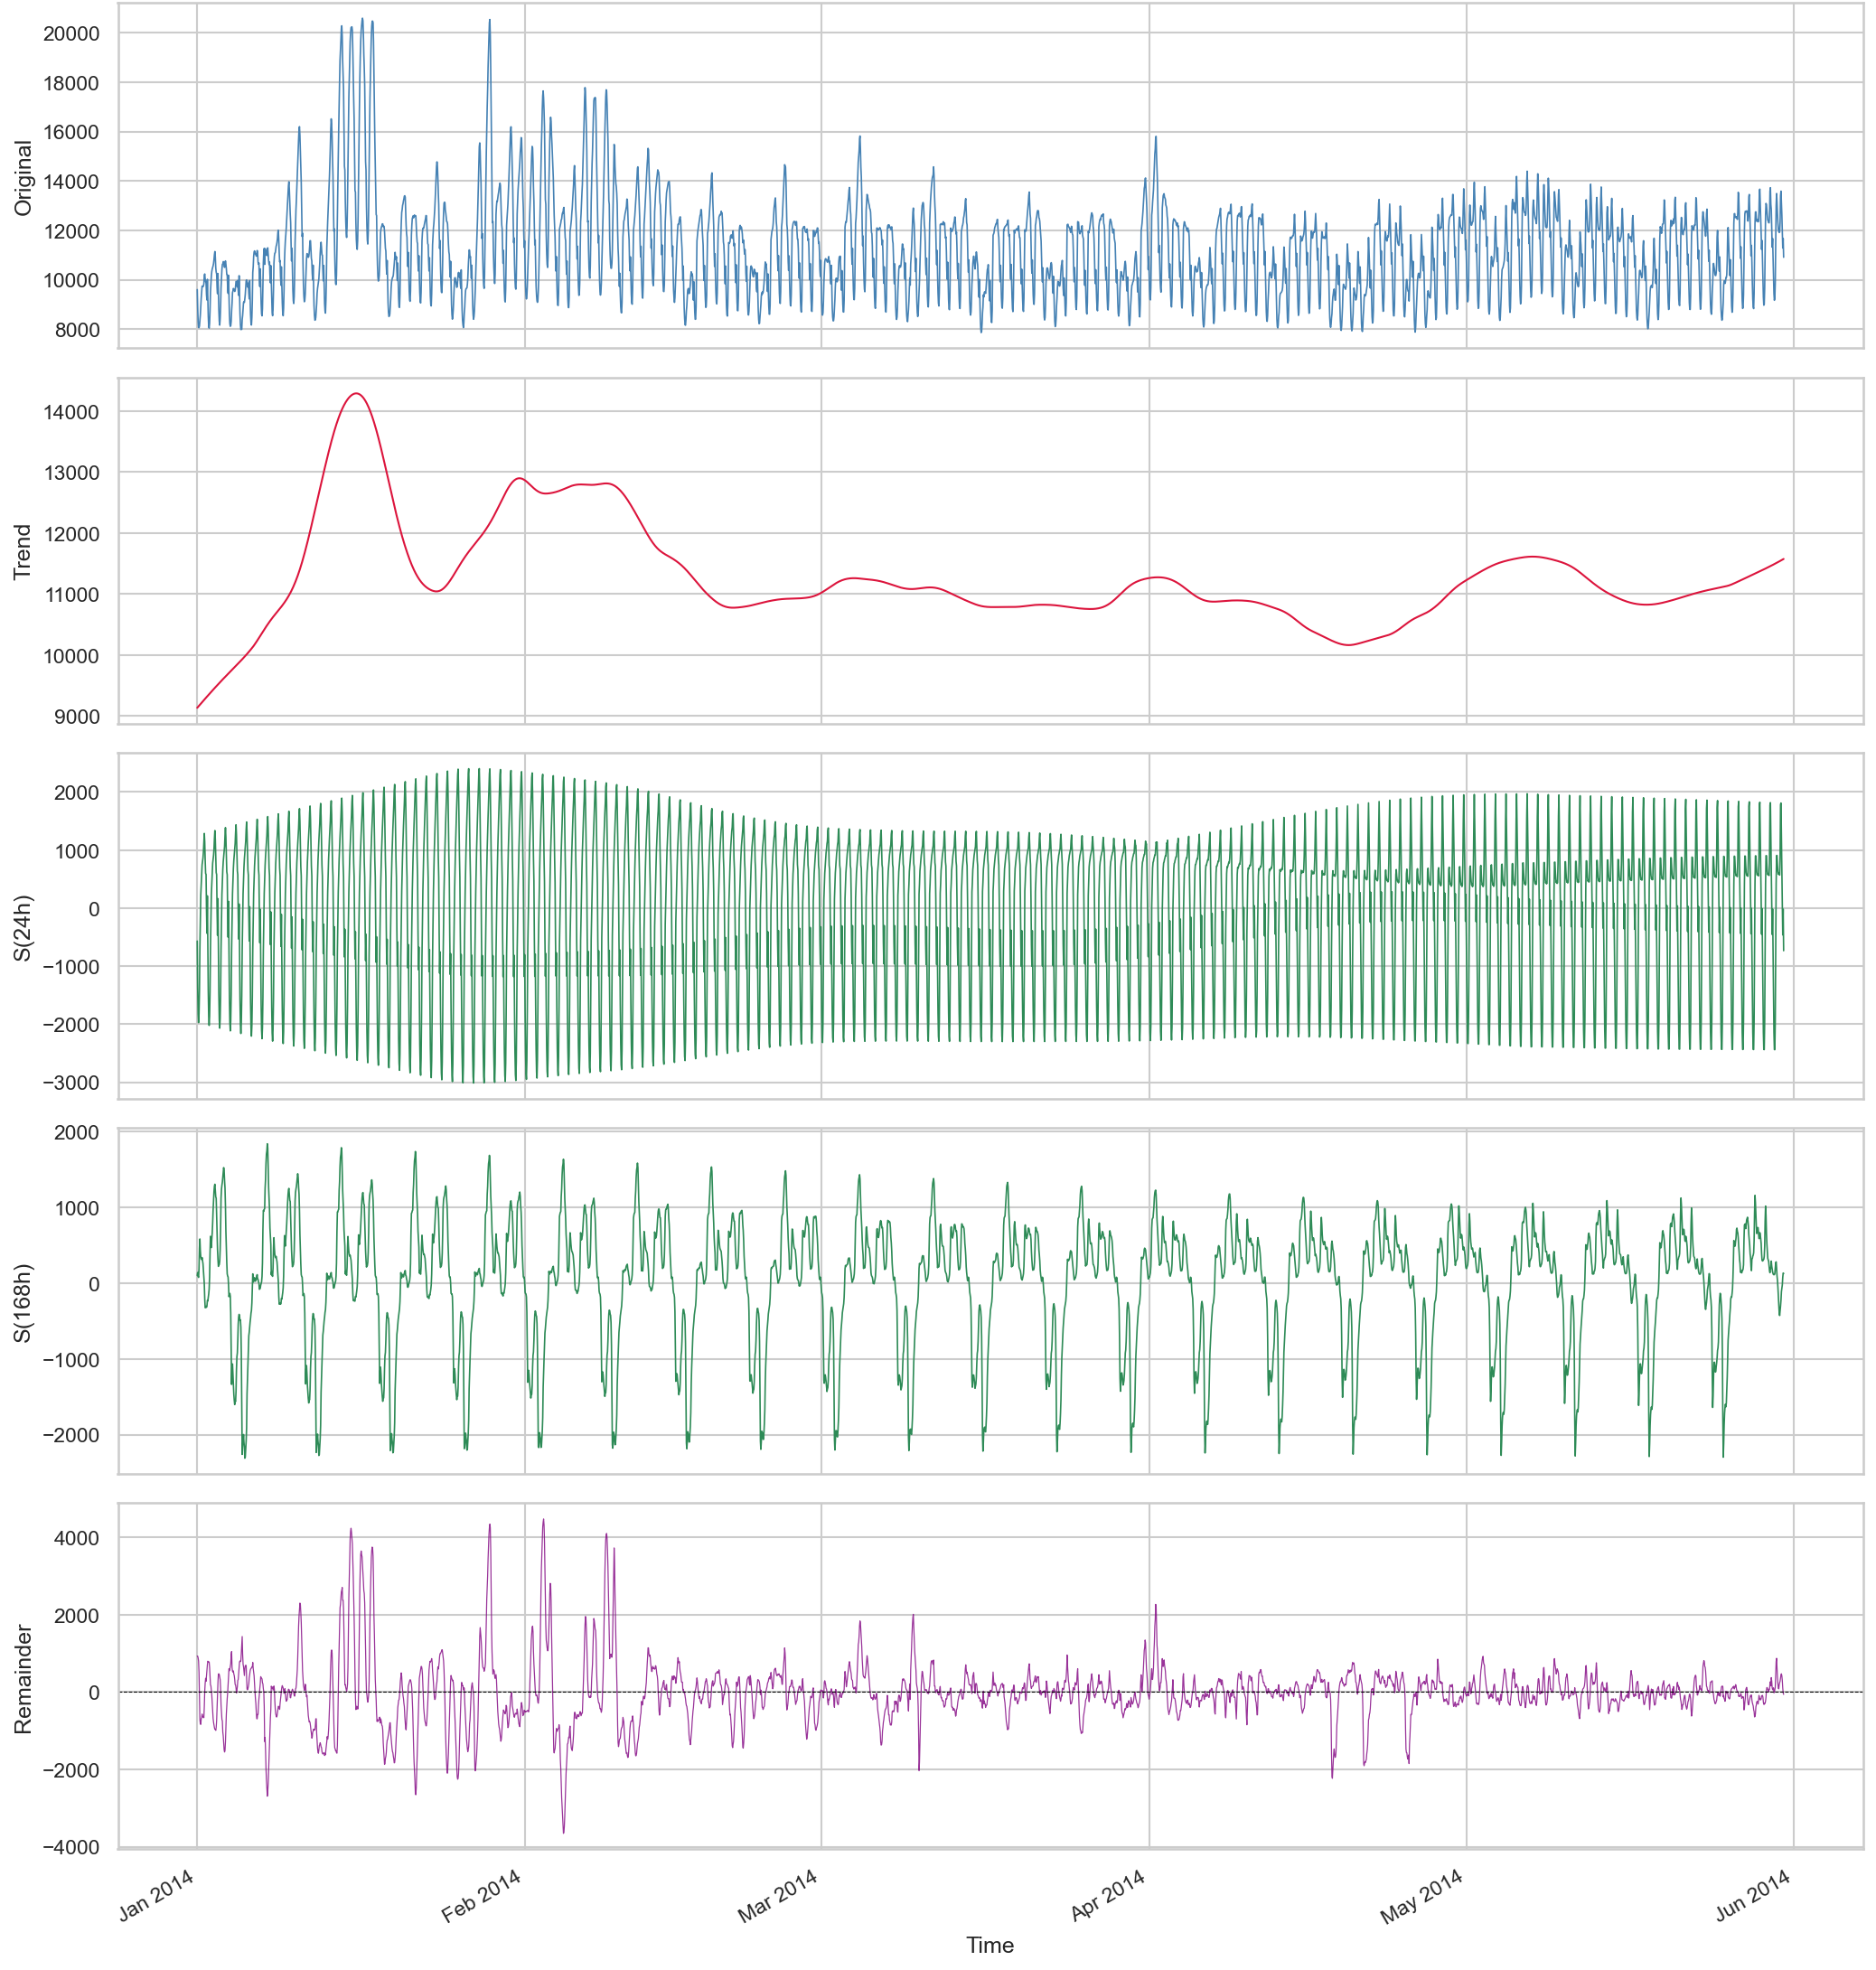
\includegraphics[width=\columnwidth]{figs/c1.png}
\caption{MSTL decomposition of Victoria electricity demand (3,601 hourly points, 1 January--31 May 2014). Rows from top: original series, trend, daily component $S_{24}$, weekly component $S_{168}$, remainder.}\label{fig:vic}
\end{figure}

\begin{figure*}[!t]
\centering
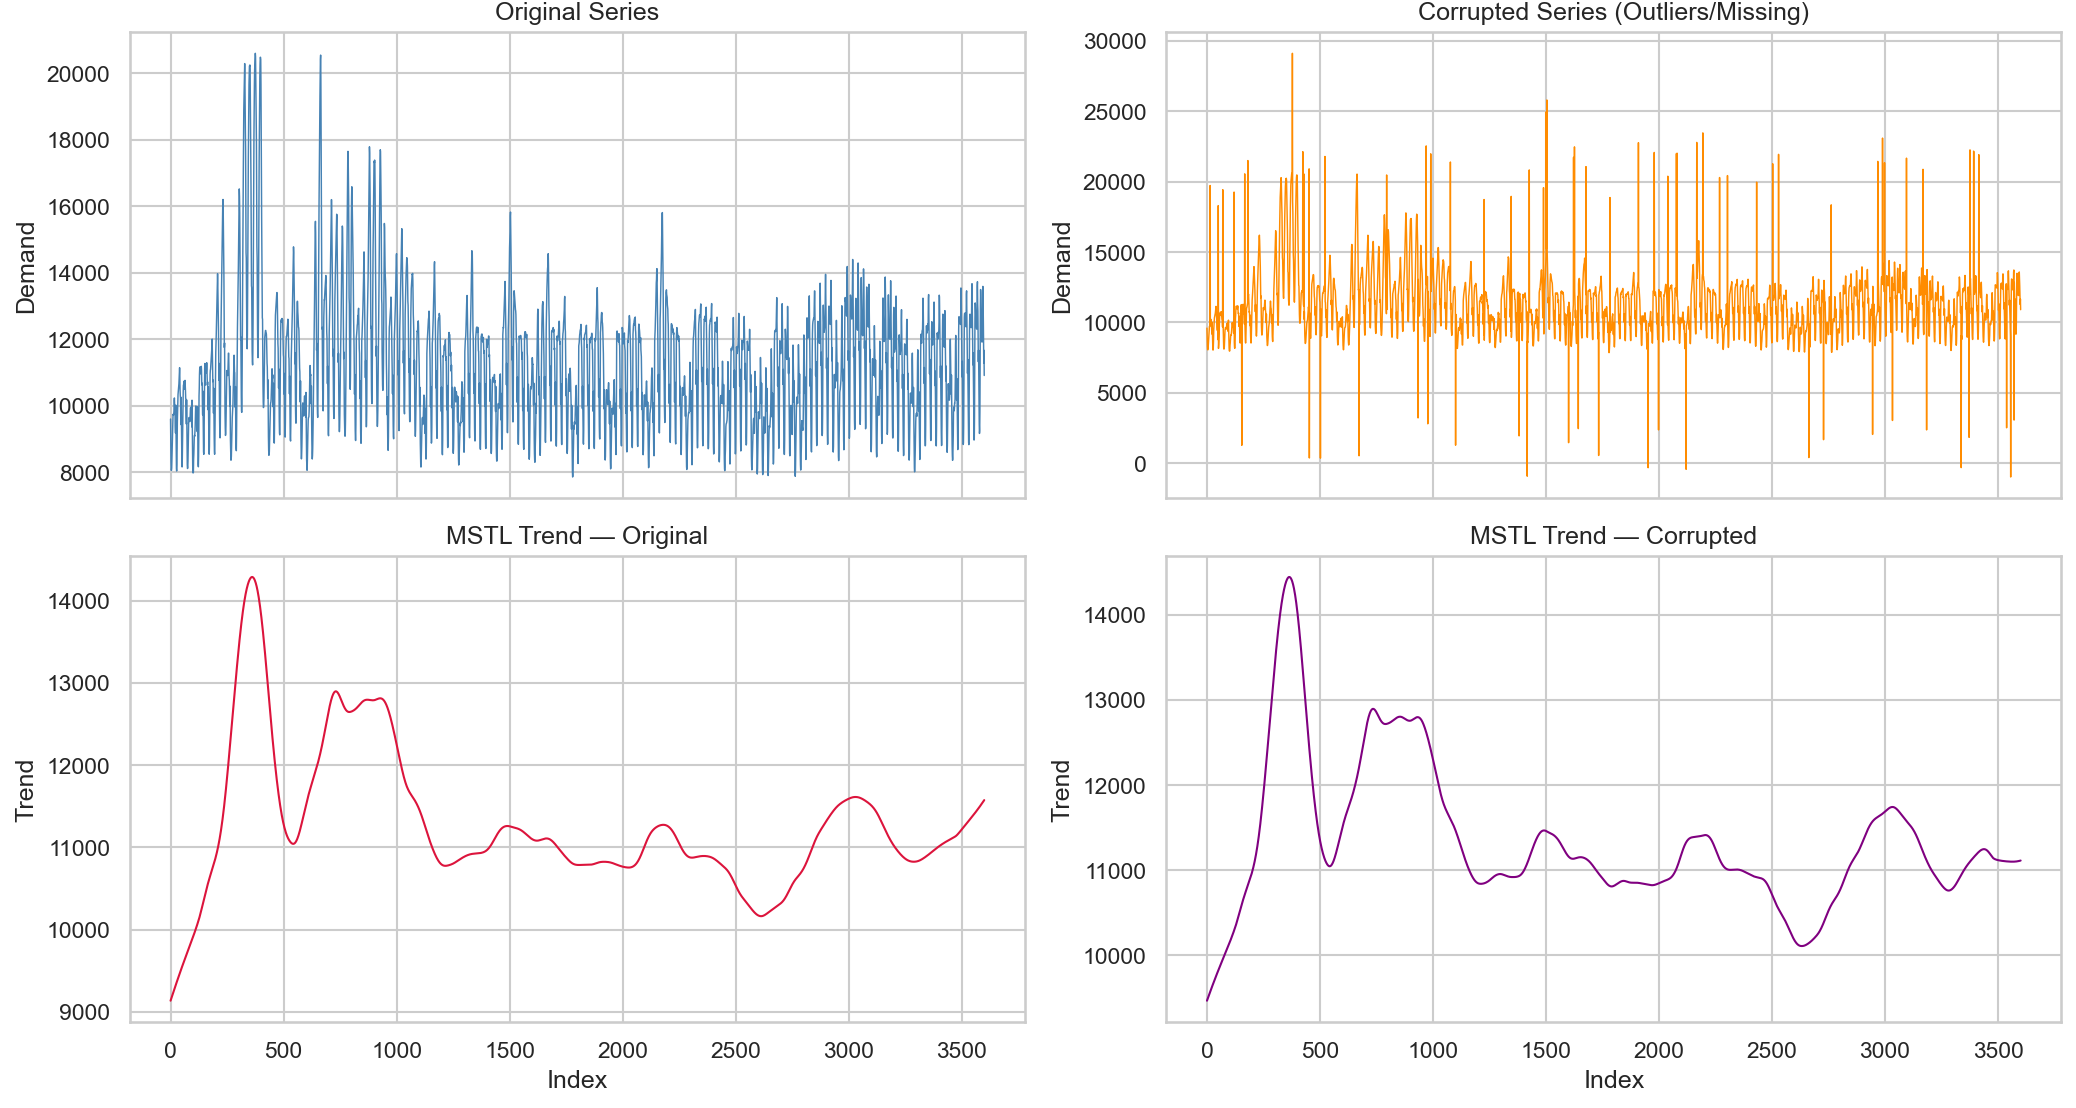
\includegraphics[width=0.78\textwidth]{figs/c3.png}
\caption{Effect of 5\% spike contamination on the series and on its estimated trend. Left: original series and clean trend. Right: corrupted series and distorted trend.}\label{fig:rob}
\end{figure*}

\section{Comparison with Other Methods}
We compared our code with the \texttt{statsmodels} implementation of MSTL, single-period STL, and TBATS (Table~\ref{tab:bench}).

\begin{table}[t]
\caption{Decomposition methods on the electricity series. ``Rem.\ std'' is the remainder standard deviation in MWh.}\label{tab:bench}
\centering\small
\begin{tabular}{@{}lcrrr@{}}
\toprule
\textsc{Method} & \textsc{Periods} & $n$ & \textsc{Time (s)} & \textsc{Rem.\ std}\\
\midrule
\textsc{Ours (MSTL)} & 24, 168 & 3601 & 0.230 & 809.77\\
\textsc{statsmodels} & 24, 168 & 3601 & 1.037 & 809.77\\
\textsc{STL} & 24 & 3601 & 0.078 & 599.38\\
\textsc{TBATS} & 24, 168 & 500 & 28.492 & 1280.40\\
\bottomrule
\end{tabular}
\end{table}

Our implementation and the library version produce the same decomposition, with trend values differing by less than 0.05\,MWh, and ours ran about 4.5 times faster. We attribute this to how LOESS parameters are passed, although we did not profile it further. TBATS needed 28.49\,s for only 500 points. Because that run used a shorter series, the timing understates the true gap rather than giving a like-for-like ratio.

\section{Synthetic Ground-Truth Test}
\begin{figure}[t]
\centering
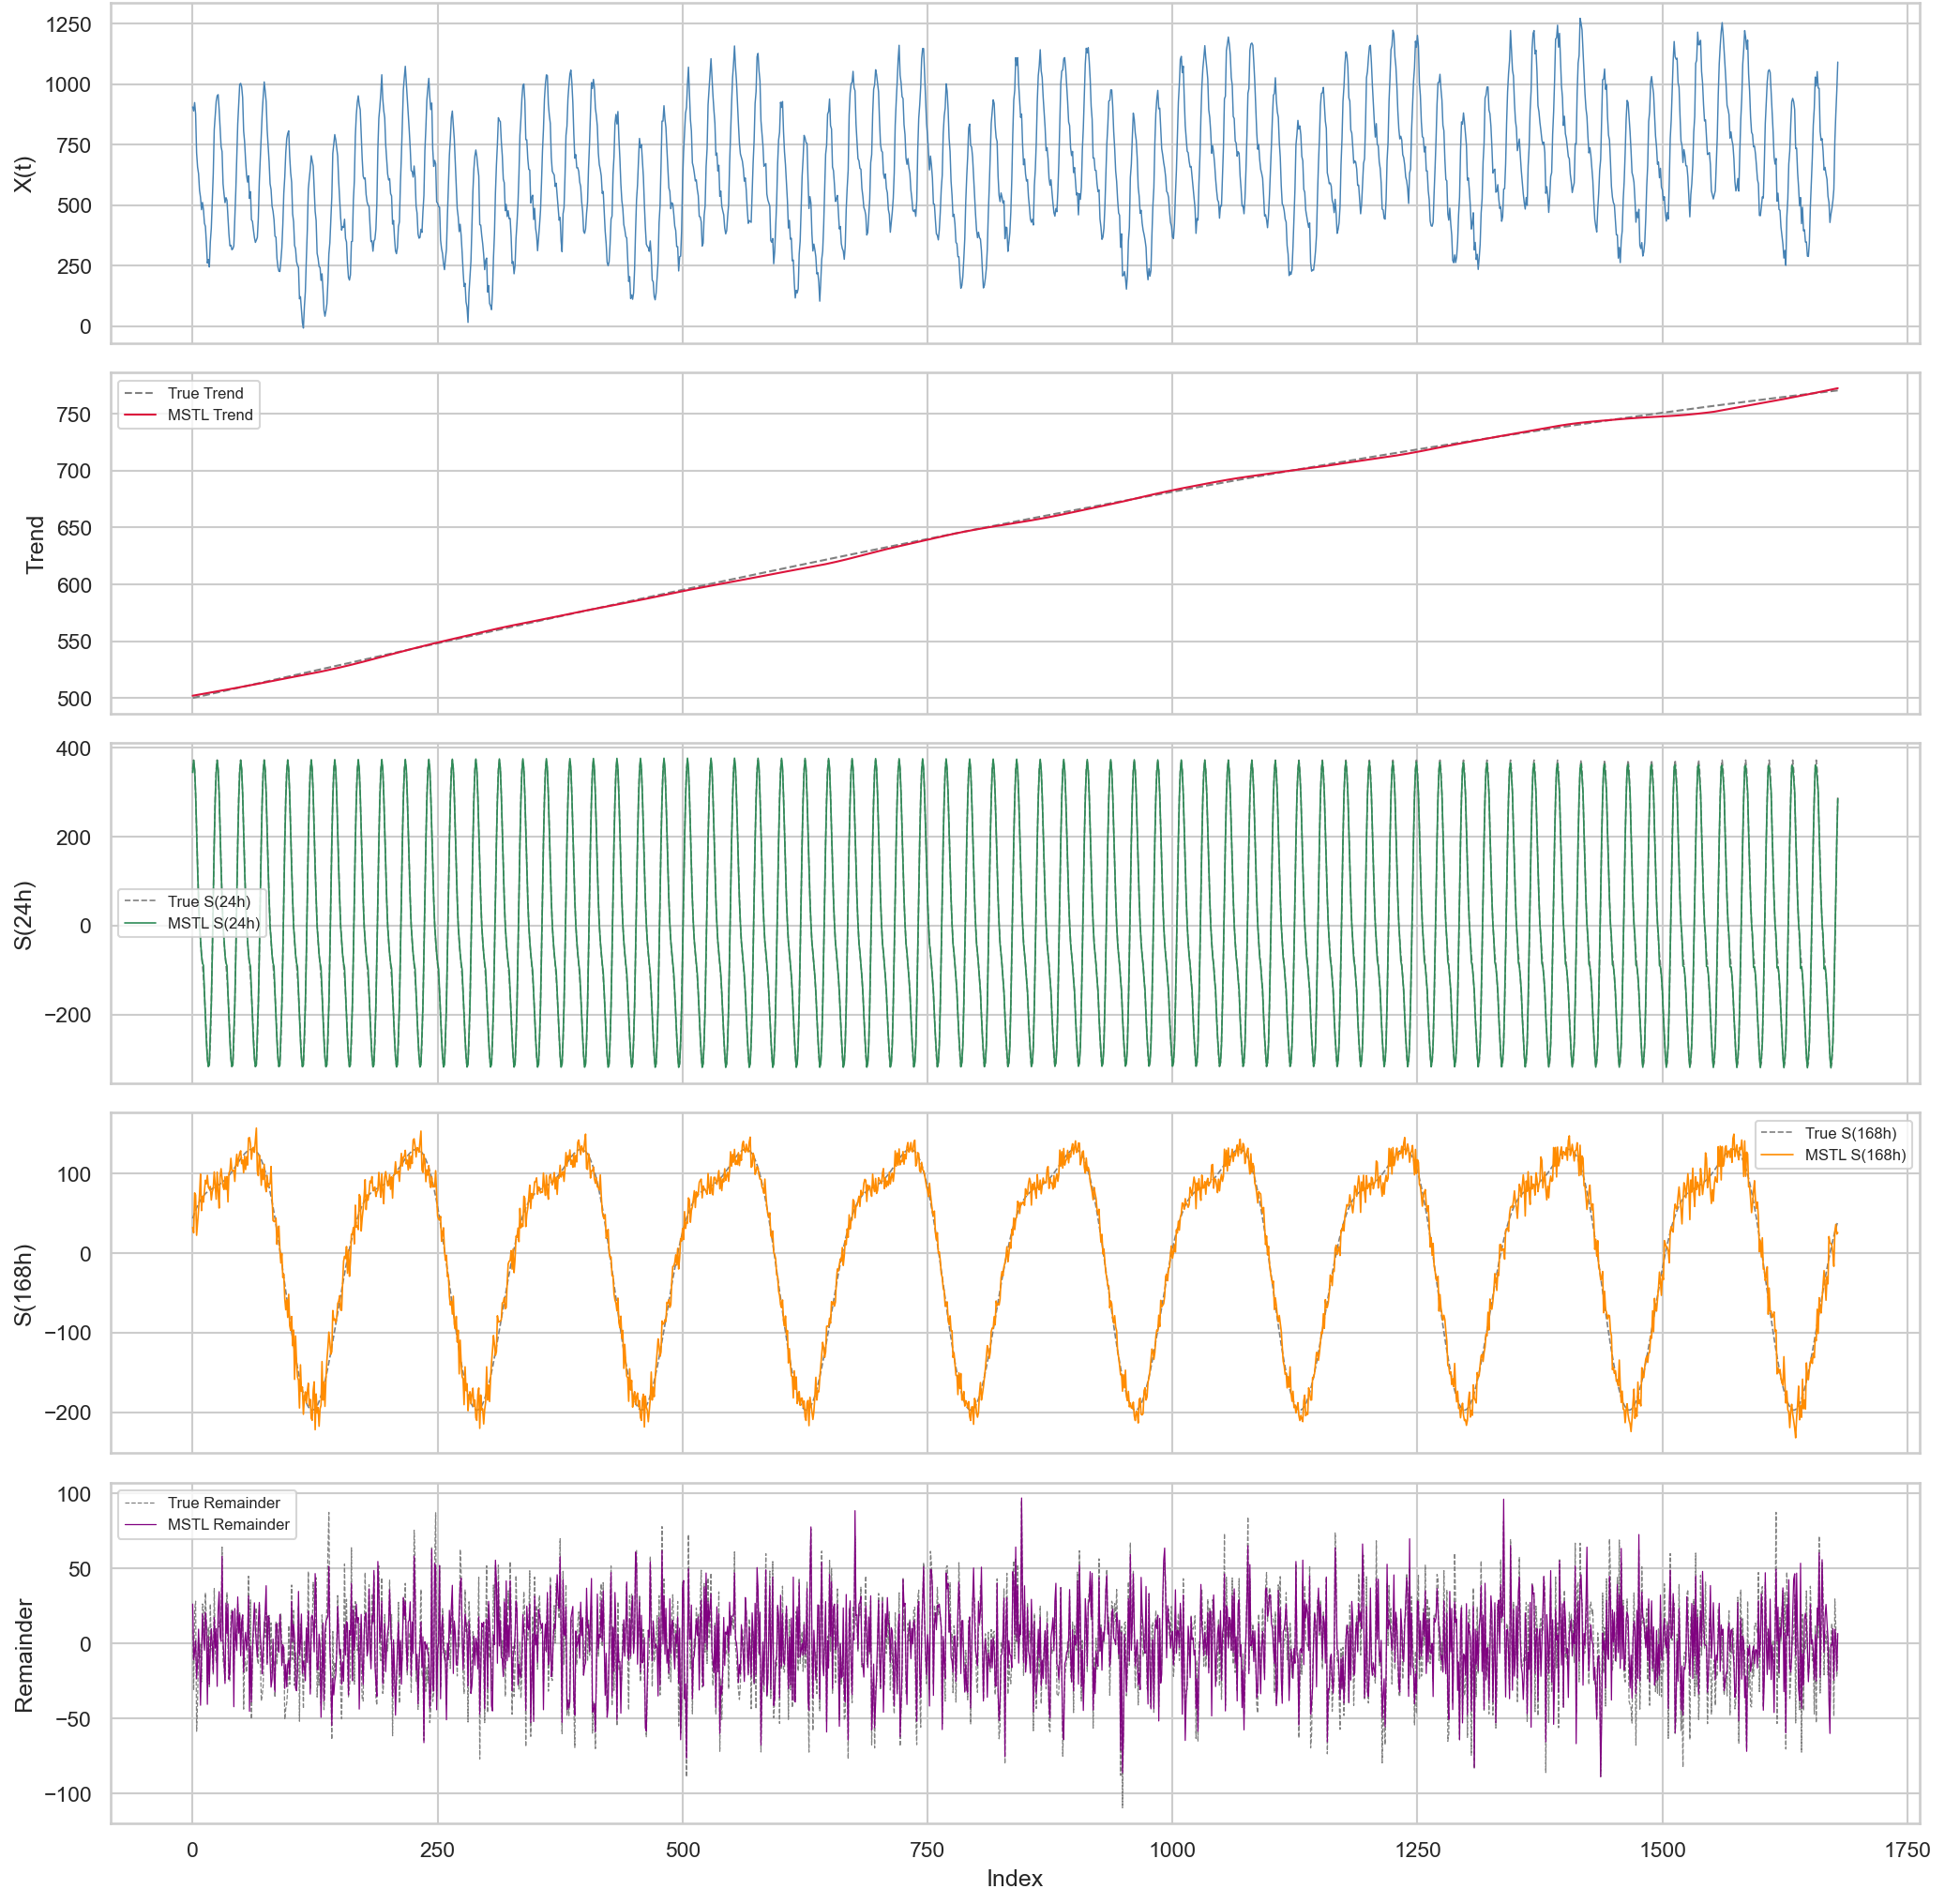
\includegraphics[width=\columnwidth]{figs/c2.png}
\caption{True components (dashed) and MSTL estimates (solid) on the synthetic series.}\label{fig:syn}
\end{figure}

Real data has no known components, so the accuracy of a decomposition cannot be measured on it directly. We therefore built a series of $n=1{,}680$ hours (70 days) from known parts:
\begin{align*}
T(t)&=500+0.05t+200\sin(2\pi t/8760),\\
S_{24}(t)&=300\sin(2\pi t/24+1)+100\cos(4\pi t/24),\\
S_{168}(t)&=150\sin(2\pi t/168)+50\cos(4\pi t/168+0.5),
\end{align*}
plus Gaussian noise $R(t)\sim\mathcal N(0,30^2)$ with seed 42. Figure~\ref{fig:syn} overlays the true and estimated components and Table~\ref{tab:syn} gives the errors.

\begin{table}[t]
\caption{Error against ground truth ($n=1{,}680$).}\label{tab:syn}
\centering\small
\begin{tabular}{@{}lccc@{}}
\toprule
\textsc{Component} & \textsc{True range} & \textsc{RMSE} & \textsc{Rel.\ error}\\
\midrule
\textsc{Trend} $T$ & [500, 650] & 1.854 & 1.24\%\\
\textsc{Daily} $S_{24}$ & [$-$320, 320] & 6.260 & 1.96\%\\
\textsc{Weekly} $S_{168}$ & [$-$165, 165] & 12.972 & 7.86\%\\
\textsc{Remainder} $R$ & $\sigma=30$ & 14.315 & ---\\
\bottomrule
\end{tabular}
\end{table}

The trend and daily cycle are recovered closely. The weekly cycle has a larger error, which we think comes from the series holding only ten weekly cycles, leaving each LOESS fit with little data.

\section{Extension Studies}
\subsection{Seasonal Window and Iterations}
We varied the seasonal LOESS window $n_s\in\{7,11,15,21,25\}$ and the number of outer iterations $I\in\{1,2,3\}$. Reconstruction error stayed below $10^{-13}$ in every case. This is expected, since the remainder is computed by subtraction, so the check validates the code rather than the statistics. Run time grew roughly linearly with iterations (0.10, 0.20, and 0.31\,s for $I=1,2,3$). Windows with $n_s\ge15$ gave smoother seasonal estimates, meaning less fitting of subseries noise.

\subsection{Ablation over Seasonal Periods}
On the electricity series we compared daily only ($m=24$), weekly only ($m=168$), and both. The weekly-only model left a remainder standard deviation of 861.03\,MWh because the daily cycle stayed in the residual. The daily-only model reached a lower 599.38\,MWh, but a spectral check showed the weekly pattern had been absorbed into the trend. The two-period model gave 809.77\,MWh. A smaller remainder is therefore not automatically better: with fewer seasonal terms, structure shifts into the trend instead of disappearing.

\subsection{Outliers and Missing Values}
We corrupted the electricity series in two ways. Removing 2\% and 10\% of the points at random raised trend RMSE by only 0.45\% and 0.89\%, since linear interpolation fills short gaps well. Adding $\pm5\sigma$ spikes to 2\%, 5\%, and 10\% of the points raised trend RMSE by 13.50\%, 23.05\%, and 33.56\% (Figure~\ref{fig:rob}). The base method has no robust re-weighting step, so large spikes pass straight into the trend.

\subsection{Scalability}
We timed the method for lengths from 168 to 3,601 hours: 0.0029\,s (168), 0.0451\,s (720), 0.0901\,s (1440), 0.1240\,s (2160), and 0.2338\,s (3601). A linear fit gives $R^2>0.998$ (Figure~\ref{fig:scale}), and peak memory stayed under 0.75\,MB.

\begin{figure}[t]
\centering
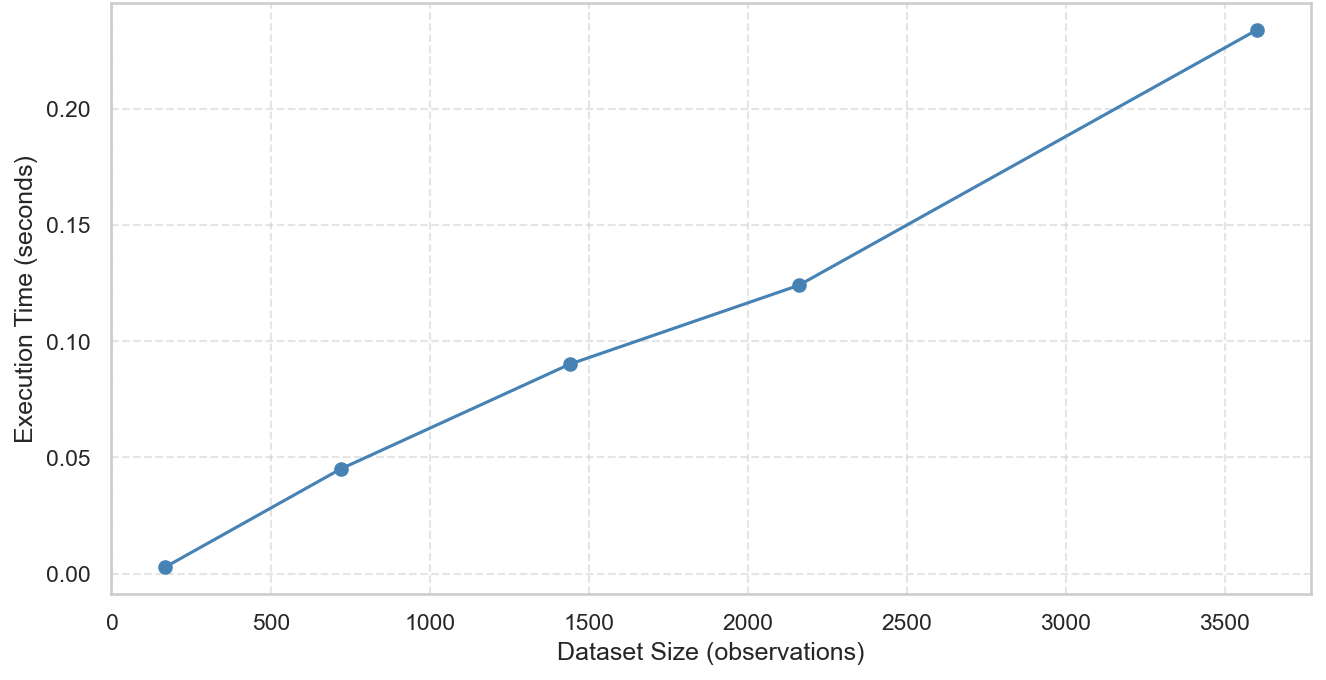
\includegraphics[width=0.92\columnwidth]{figs/c4.png}
\caption{Wall-clock time against series length.}\label{fig:scale}
\end{figure}

\section{Conclusion}
We implemented MSTL, reproduced the Victoria electricity decomposition, and checked the method against known components. It scales linearly and tolerates missing values, but it is sensitive to spike outliers. Adding the outer-loop robustness weights of STL, or filtering outliers before decomposition, is a natural next step for production pipelines.

\begingroup\small
\begin{thebibliography}{9}
\bibitem[Bandara et al.(2021)Bandara, Hyndman, and Bergmeir]{bandara2021}
Bandara, K., Hyndman, R.~J., and Bergmeir, C. MSTL: A seasonal-trend decomposition algorithm for time series with multiple seasonal patterns. \emph{arXiv preprint arXiv:2107.13462}, 2021. Also in \emph{International Journal of Operational Research}, 52(1):79--98, 2025.
\bibitem[Box \& Cox(1964)Box and Cox]{box1964}
Box, G.~E.~P. and Cox, D.~R. An analysis of transformations. \emph{Journal of the Royal Statistical Society: Series B}, 26(2):211--252, 1964.
\bibitem[Cleveland et al.(1990)Cleveland, Cleveland, McRae, and Terpenning]{cleveland1990}
Cleveland, R.~B., Cleveland, W.~S., McRae, J.~E., and Terpenning, I. STL: A seasonal-trend decomposition procedure based on LOESS. \emph{Journal of Official Statistics}, 6(1):3--73, 1990.
\bibitem[Cleveland(1979)]{cleveland1979}
Cleveland, W.~S. Robust locally weighted regression and smoothing scatterplots. \emph{Journal of the American Statistical Association}, 74(368):829--836, 1979.
\bibitem[De~Livera et al.(2011)De~Livera, Hyndman, and Snyder]{delivera2011}
De~Livera, A.~M., Hyndman, R.~J., and Snyder, R.~D. Forecasting time series with complex seasonal patterns using exponential smoothing. \emph{Journal of the American Statistical Association}, 106(496):1513--1527, 2011.
\bibitem[Hyndman \& Athanasopoulos(2018)Hyndman and Athanasopoulos]{hyndman2018}
Hyndman, R.~J. and Athanasopoulos, G. \emph{Forecasting: Principles and Practice}. OTexts, Melbourne, Australia, 2nd edition, 2018.
\bibitem[Taylor \& Letham(2018)Taylor and Letham]{taylor2018}
Taylor, S.~J. and Letham, B. Forecasting at scale. \emph{The American Statistician}, 72(1):37--45, 2018.
\end{thebibliography}
\endgroup
\end{document}
